\documentclass[11pt,a4paper]{article}

\usepackage[left=2cm,right=2cm,top=2cm,bottom=2cm]{geometry}
\setlength{\parindent}{0pt}
\setlength{\parskip}{5pt plus 1pt}

\usepackage[T1]{fontenc}
\usepackage[utf8]{inputenc}
\usepackage{lmodern,microtype}
\usepackage{amsmath,amssymb}
\usepackage{tikz}
\usetikzlibrary{arrows.meta,positioning}
\usepackage{enumitem}

\usepackage{fancyhdr}
\pagestyle{fancy}
\fancyhf{}
\renewcommand{\headrulewidth}{0.6pt}
\lhead{\small\textbf{CS5800 -- Algorithms}}
\rhead{\small\textbf{Group Seminar -- Problem Set}}
\cfoot{\small\thepage}

\tikzset{
  nd/.style={circle,draw,minimum size=16pt,inner sep=0pt,font=\small\bfseries},
  sn/.style={nd,draw=teal,fill=teal!10},
  tn/.style={nd,draw=red!70,fill=red!8},
  ed/.style={-{Stealth[length=4pt,width=3pt]},semithick},
}

\begin{document}

\begin{center}
{\Large\bfseries Maximum Flow -- Problem Set}\\[4pt]
{\small Ford-Fulkerson Algorithm \& Max-Flow Min-Cut Theorem}
\end{center}

\bigskip

% ============================================================
\textbf{\large Problem 1: Irrigation Canal System}
\medskip

A farmer is designing an irrigation system for his fields. Water is pumped from a reservoir (node~1) and must reach a storage tank (node~5) through a network of canals. Each canal allows water to flow in one direction only, and the label on each edge represents the maximum flow rate of that canal (in liters per second). Note that there may be multiple canals between the same pair of junctions.

\begin{center}
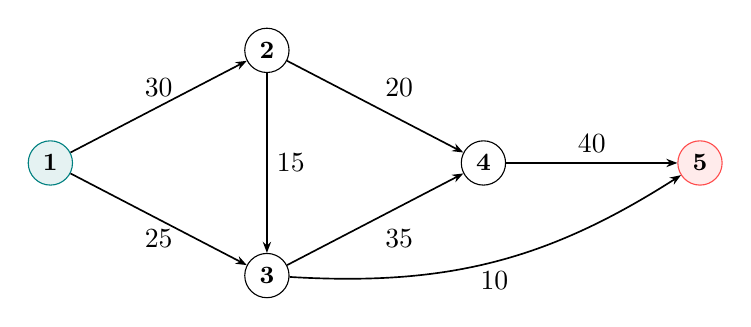
\begin{tikzpicture}[scale=1.1]
  \node[sn] (1) at (0,0) {1};
  \node[nd] (2) at (2.5,1.3) {2};
  \node[nd] (3) at (2.5,-1.3) {3};
  \node[nd] (4) at (5,0) {4};
  \node[tn] (5) at (7.5,0) {5};

  \draw[ed] (1) -- node[above]{30} (2);
  \draw[ed] (1) -- node[below]{25} (3);
  \draw[ed] (2) -- node[above right]{20} (4);
  \draw[ed] (2) -- node[right]{15} (3);
  \draw[ed] (3) -- node[below right]{35} (4);
  \draw[ed] (4) -- node[above]{40} (5);
  \draw[ed] (3) to[bend right=18] node[below]{10} (5);
\end{tikzpicture}
\end{center}

\begin{enumerate}[label=(\alph*)]
  \item Compute the maximum flow from node~1 to node~5 using the Ford-Fulkerson algorithm with BFS. For each iteration, clearly state: the augmenting path, the bottleneck capacity along that path, and the total flow after the update.

  \item Write down the final flow value on every edge. Verify that flow conservation holds at each intermediate node (2, 3, and~4).

  \item Identify the minimum cut $(S, T)$ by examining which nodes are reachable from node~1 in the final residual network. List the cut edges and verify that the cut capacity equals the maximum flow.

  \item The farmer considers building one additional canal from node~3 to node~2 with capacity~$k$. For what values of $k$ (if any) would this new canal increase the maximum flow? If the maximum flow can be increased, what is the new maximum flow? Justify your answer.
\end{enumerate}

\newpage

% ============================================================
\textbf{\large Problem 2: Network Reliability Analysis}
\medskip

Consider the following flow network where each edge has the indicated capacity.

\begin{center}
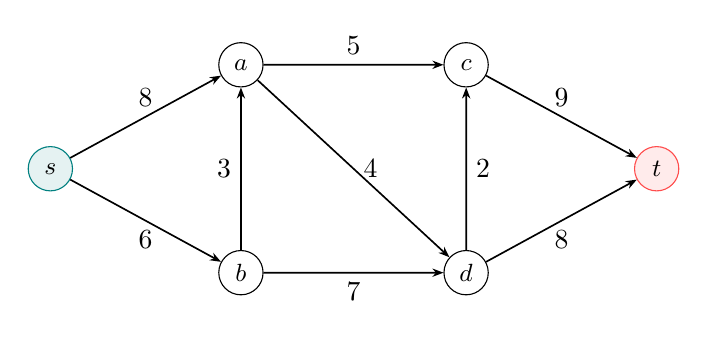
\begin{tikzpicture}[scale=1.1]
  \node[sn] (s) at (0,0) {$s$};
  \node[nd] (a) at (2.2,1.2) {$a$};
  \node[nd] (b) at (2.2,-1.2) {$b$};
  \node[nd] (c) at (4.8,1.2) {$c$};
  \node[nd] (d) at (4.8,-1.2) {$d$};
  \node[tn] (t) at (7,0) {$t$};

  \draw[ed] (s) -- node[above]{8} (a);
  \draw[ed] (s) -- node[below]{6} (b);
  \draw[ed] (a) -- node[above]{5} (c);
  \draw[ed] (a) -- node[right]{4} (d);
  \draw[ed] (b) -- node[left]{3} (a);
  \draw[ed] (b) -- node[below]{7} (d);
  \draw[ed] (c) -- node[above]{9} (t);
  \draw[ed] (d) -- node[below]{8} (t);
  \draw[ed] (d) -- node[right]{2} (c);
\end{tikzpicture}
\end{center}

\begin{enumerate}[label=(\alph*)]
  \item Find the maximum flow from $s$ to $t$. Show your work by running Ford-Fulkerson with BFS.

  \item Someone claims that the flow $f$ defined by $f(s,a)=5$, $f(s,b)=6$, $f(a,c)=5$, $f(b,d)=6$, $f(c,t)=5$, $f(d,t)=6$, and all other edge flows equal to~0, is a maximum flow. Without running the algorithm again, prove or disprove this claim. (\textit{Hint: examine the residual network.})

  \item Find \emph{all} minimum cuts in this network. Prove that you have found them all. (\textit{Hint: there may be more than one.})

  \item Suppose we remove the edge $d \to c$ (capacity~2) from the network. Does the maximum flow change? Prove your answer without re-running Ford-Fulkerson from scratch.
\end{enumerate}

\newpage

% ============================================================
\begin{center}
{\Large\bfseries Solutions}
\end{center}

\bigskip

\textbf{\large Problem 1 Solution}
\medskip

\textbf{(a)} We apply Ford-Fulkerson with BFS on the given network.

\textit{Iteration 1.} BFS finds shortest path $1 \to 3 \to 5$ (2 edges).\\
Residual capacities along path: $25, 10$. Bottleneck: $\min(25, 10) = 10$.\\
Push flow 10. Running total: $|f| = 10$.

\textit{Iteration 2.} Edge $3\to 5$ is now saturated, so BFS finds $1 \to 2 \to 4 \to 5$ (3 edges).\\
Residual capacities: $30, 20, 40$. Bottleneck: $\min(30, 20, 40) = 20$.\\
Push flow 20. Running total: $|f| = 30$.

\textit{Iteration 3.} BFS finds $1 \to 3 \to 4 \to 5$ (3 edges).\\
Residual capacities: $25-10=15, 35, 40-20=20$. Bottleneck: $\min(15, 35, 20) = 15$.\\
Push flow 15. Running total: $|f| = 45$.

\textit{Iteration 4.} Edge $1\to 3$ is now saturated. BFS finds $1 \to 2 \to 3 \to 4 \to 5$ (4 edges).\\
Residual capacities: $30-20=10, 15, 35-15=20, 20-15=5$. Bottleneck: $\min(10, 15, 20, 5) = 5$.\\
Push flow 5. Running total: $|f| = 50$.

\textit{Termination.} BFS from node~1: $1\to 2$ (res $5$), $2\to 3$ (res $10$), $2\to 4$ (res $0$), $3\to 4$ (res $15$), $4\to 5$ (res $0$), $3\to 5$ (res $0$). Reachable set $\{1,2,3,4\}$; node~5 unreachable.

No augmenting path exists. \textbf{Maximum flow = 50.}

\medskip

\textbf{(b)} Final edge flows:

\begin{center}
\begin{tabular}{lcccccc}
Edge & $1\to 2$ & $1\to 3$ & $2\to 4$ & $2\to 3$ & $3\to 4$ & $3\to 5$ \\
\hline
Flow / Capacity & 25/30 & 25/25 & 20/20 & 5/15 & 20/35 & 10/10 \\[4pt]
Edge & $4\to 5$ \\
\cline{1-2}
Flow / Capacity & 40/40
\end{tabular}
\end{center}

Conservation check:
\begin{itemize}[nosep]
  \item Node 2: in $= f(1,2) = 25$. Out $= f(2,4) + f(2,3) = 20 + 5 = 25$. \checkmark
  \item Node 3: in $= f(1,3) + f(2,3) = 25 + 5 = 30$. Out $= f(3,4) + f(3,5) = 20 + 10 = 30$. \checkmark
  \item Node 4: in $= f(2,4) + f(3,4) = 20 + 20 = 40$. Out $= f(4,5) = 40$. \checkmark
\end{itemize}

\medskip

\textbf{(c)} From the termination analysis in part (a), the reachable set from node~1 in $G_f$ is $S = \{1, 2, 3, 4\}$ and $T = \{5\}$.

Cut edges ($S \to T$):
\begin{itemize}[nosep]
  \item $4 \to 5$: capacity 40
  \item $3 \to 5$: capacity 10
\end{itemize}

Cut capacity $= 40 + 10 = 50 = |f^*|$. \checkmark

\medskip

\textbf{(d)} The minimum cut has $S = \{1,2,3,4\}$ and $T = \{5\}$, with cut edges $4\to 5$ (cap 40) and $3\to 5$ (cap 10).

A new canal $3 \to 2$ with capacity $k$ connects two nodes both in $S$. Since both endpoints are on the source side of the min-cut, this edge does not cross any cut and cannot increase the capacity of the minimum cut $\{1,2,3,4\}$ vs.\ $\{5\}$.

However, could a different cut become the new bottleneck? Consider cut $S'=\{1\}$, $T'=\{2,3,4,5\}$: capacity $= c(1,2)+c(1,3) = 30+25=55$. Adding $3\to 2$ does not affect this (both in $T'$). For any other cut, the new edge either has both endpoints on the same side or goes from $T$ to $S$ (which doesn't count).

Since no cut's capacity is affected by adding $3\to 2$, the maximum flow remains 50 for all values of $k$. \textbf{The new canal cannot increase the maximum flow.}

\newpage

\textbf{\large Problem 2 Solution}
\medskip

\textbf{(a)} Ford-Fulkerson with BFS on the given network:

\textit{Iteration 1.} Path $s \to a \to c \to t$. Bottleneck: $\min(8, 5, 9) = 5$. Total: $|f|=5$.

\textit{Iteration 2.} Path $s \to b \to d \to t$. Bottleneck: $\min(6, 7, 8) = 6$. Total: $|f|=11$.

\textit{Iteration 3.} Path $s \to a \to d \to t$. Residual: $8-5=3, 4, 8-6=2$. Bottleneck: $\min(3,4,2)=2$. Total: $|f|=13$.

\textit{Iteration 4.} Path $s \to a \to d \to c \to t$.
Residual: $8-7=1, 4-2=2, 2, 9-5=4$. Bottleneck: $\min(1,2,2,4)=1$. Total: $|f|=14$.

\textit{Iteration 5.} Check reachability from $s$ in $G_f$: $s\to a$ (res $8-8=0$), $s\to b$ (res $6-6=0$). Neither $a$ nor $b$ is reachable. No augmenting path.

\textbf{Maximum flow = 14.}

Final flows: $f(s,a)=8$, $f(s,b)=6$, $f(a,c)=5$, $f(a,d)=3$, $f(b,a)=0$, $f(b,d)=6$, $f(d,c)=1$, $f(c,t)=6$, $f(d,t)=8$.

\medskip

\textbf{(b)} The claimed flow has value $|f'|=5+6=11$. We construct the residual network $G_{f'}$:

Forward residual edges with $c_f > 0$: $s\to a$: $8-5=3$, $a\to d$: $4$, $b\to a$: $3$, $b\to d$: $7-6=1$, $d\to c$: $2$, $c\to t$: $9-5=4$, $d\to t$: $8-6=2$.

BFS from $s$: $s \to a$ (res $3$) $\to d$ (res $4$) $\to t$ (res $2$). This is an augmenting path with bottleneck $\min(3,4,2)=2$.

Since an augmenting path exists in $G_{f'}$, the flow $f'$ is \textbf{not maximum}. The claim is false.
\medskip

\textbf{(c)} From part (a), the final residual has $S_1 = \{s\}$ (neither $a$ nor $b$ reachable), so $(S_1, T_1) = (\{s\}, \{a,b,c,d,t\})$ is a min-cut with capacity $8+6=14$.

To find all min-cuts, we look for other cuts with capacity exactly 14. For a cut $(S,T)$ with $s\in S$ and $t\in T$:

\begin{itemize}[nosep]
\item $S=\{s,a\}$: cut edges $s\to b$ (6), $a\to c$ (5), $a\to d$ (4). Capacity $=15\neq 14$.
\item $S=\{s,b\}$: cut edges $s\to a$ (8), $b\to a$ (3), $b\to d$ (7). Capacity $=18\neq 14$.
\item $S=\{s,a,b\}$: cut edges $a\to c$ (5), $a\to d$ (4), $b\to d$ (7). Capacity $=16\neq 14$.
\item $S=\{s,a,d\}$: cut edges $s\to b$ (6), $a\to c$ (5), $d\to c$ (2), $d\to t$ (8). Capacity $=21$.
\item $S=\{s,a,b,d\}$: cut edges $a\to c$ (5), $d\to c$ (2), $d\to t$ (8), $b$ has no edge to $T\setminus\{a,d\}$... $b\to a$: both in $S$. Edges to $T=\{c,t\}$: $a\to c$ (5), $d\to c$ (2), $d\to t$ (8). Capacity $=15$.
\item $S=\{s,a,b,c\}$: $T=\{d,t\}$. Cut edges: $a\to d$ (4), $b\to d$ (7), $c\to t$ (9). Capacity $=20$.
\item $S=\{s,a,b,c,d\}$: $T=\{t\}$. Cut edges: $c\to t$ (9), $d\to t$ (8). Capacity $=17$.
\end{itemize}

(Other combinations with $s\in S$ can be checked similarly; none yield capacity 14.)

The \textbf{unique minimum cut} is $(\{s\}, \{a,b,c,d,t\})$ with capacity 14.
\medskip

\textbf{(d)} In our maximum flow from part (a), the edge $d\to c$ carries flow $f(d,c)=1$.

If we remove $d\to c$, that 1 unit of flow is lost. The question is whether it can be rerouted. In the original solution, this flow came from the path $s\to a\to d\to c\to t$ (iteration~4). Without edge $d\to c$, that augmenting path does not exist.

After removing $d\to c$, start from the max flow of iterations 1--3 ($|f|=13$). In the residual network at that point: $s\to a$ has residual $8-7=1$, and from $a$, the only option is $a\to d$ (res $4-2=2$). From $d$: $d\to t$ has residual $8-8=0$ and $d\to c$ no longer exists. Via back-edge $d\to b$ (res $6$), then $b\to s$ back-edge --- this doesn't help reach $t$.

So no augmenting path exists at $|f|=13$ without $d\to c$.

The new maximum flow is $\mathbf{13}$, which is one less than before. The removal of $d\to c$ decreases the maximum flow by exactly 1.
\end{document}
